\section{Test Scenarios}
The purpose of this section is to highlight the findings in the various simulation runs which were performed.

The primary purpose of the simulation was to test the effect of the DOGS system. 
As part of this tests were performed to discover the effect of bus priority and to determine whether DOGS with its varying cycle time can outperform a fixed cycle time but properly coordinated offsets.

All simulations were fitted to the traffic observed in the morning period fra 7-9 am.
To account for fluctuations each test was run 10 times with different seeds.

The results of the tests are measured by extraction of average queues and delays for each intersection. This is done by inserting a node with node evaluation enabled for each of the twelve intersections.

The overall conclusion is that the combined performance of the network is reduced when DOGS is running. This means that the positive effect for traffic traversing the arterial does not outweigh the penalties for crossing traffic.

For bus priority, although it is only enabled for a few of the involved intersections - and that the implemented priority logic could be more aggressive - there is a noticable effect.

\subsection{The Effect of DOGS}
This test covers four scenarios:

\begin{enumerate}
\item DOGS and bus priority
\item DOGS without bus priority
\item Default program with bus priority
\item Default program with no priority for buses
\end{enumerate}

In scenario 1 and 2 DOGS is enabled and the capacity in the main direction is adjusted according to detector values. In scenarios 3 and 4 DOGS is disabled effectively ignoring all detections (except for buses in scenario 3) and thus the signals will remain in the base program.

As DOGS will naturally cause decreased performance for the minor roads it was decided to split the dataset so that \textit{arterial} and \textit{crossing} traffic can be distinguished. Arterial traffic is defined as traffic which enters an intersection from north or south and makes a throughgoing motion rather than turning off the arterial. All other traffic is marked as crossing.

\subsubsection*{Queue}
The average queue length indicates the number of vehicles waiting to cross an intersection ie. perform some turning motion in the beginning of the green interval. 

When queues become too long \textit{spillback} occurs causing queues upstream. In the extreme event queues stretch back to the last upstream intersection blocking all entry into the intersection and effectively causes a gridlock.
Another spillback situation, although less severe - but more common, is when vehicles waiting for a left-turn fill up a dedicated left-turning lane and spill back into the main direction.

These situations are, of course, not desirable and thus the queue length is an important factor to observe.

The way DOGS work we can make some speculations on how queues will form. The intention of DOGS is to improve the conditions for the arterial traffic, admittedly sacrificing some performance for the side roads. So we expect queues to shorter for the main direction and longer for the side roads.

\begin{figure}[ht]

    \begin{minipage}[b]{0.5\linewidth}

\begin{center}
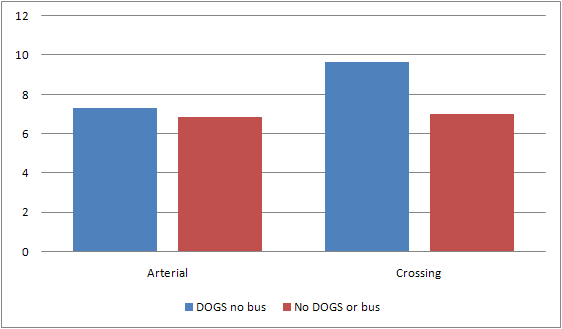
\includegraphics[scale=0.30]{aveq.png} 
\end{center}
\caption{Average queue lengths for arterial and crossing traffic}
\label{fig:aveq}

    \end{minipage}
    \hspace{0.5cm}
    \begin{minipage}[b]{0.5\linewidth}

\begin{center}
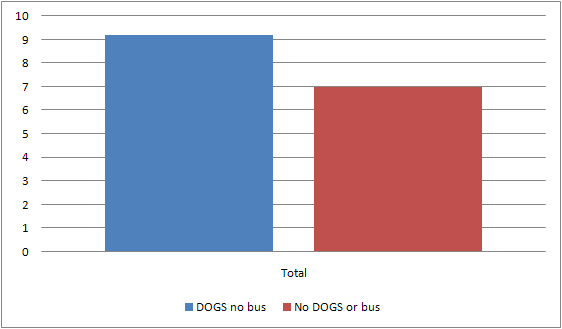
\includegraphics[scale=0.30]{aveq_total.png} 
\end{center}
\caption{Average queue lengths for all traffic types}
\label{fig:aveq_tot}

    \end{minipage}

\end{figure}

In Figures \ref{fig:aveq} and \ref{fig:aveq_tot} we see the average queue lengths for all intersections with and without DOGS, in both cases with no bus priority (since bus priority may cause increased queues and we want to save this aspect for later).

We see that DOGS severely penalizes crossing and the arterial traffic even suffers at the same time in the average case. To further inspect this phenomenon we observe Figures (\ref{fig:aveq_int_cross}-\ref{fig:aveq_int_tot}) where the average queue lengths are shown per intersection.

\begin{figure}[ht]
\begin{center}
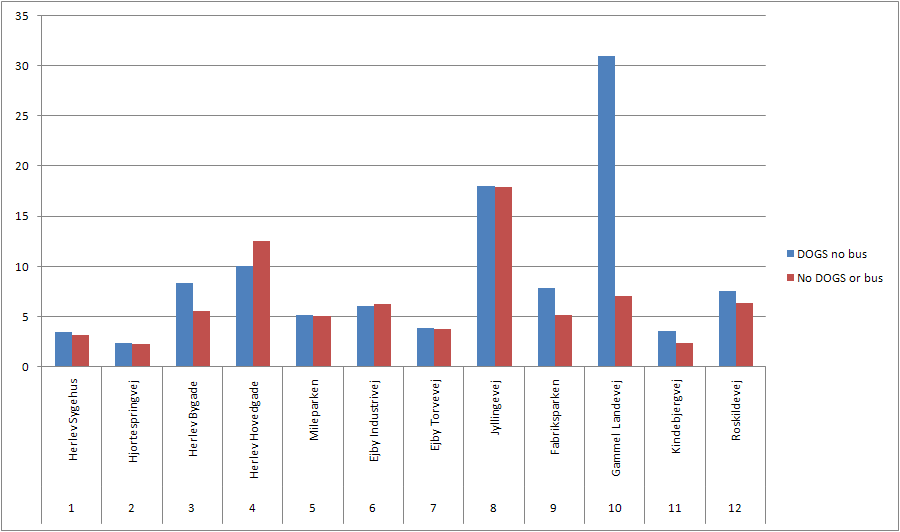
\includegraphics[scale=0.30]{aveq_intersection_crossing.png} 
\end{center}
\caption{Average queue lengths per intersection for crossing traffic}
\label{fig:aveq_int_cross}
\end{figure}

\begin{figure}[ht]
\begin{center}
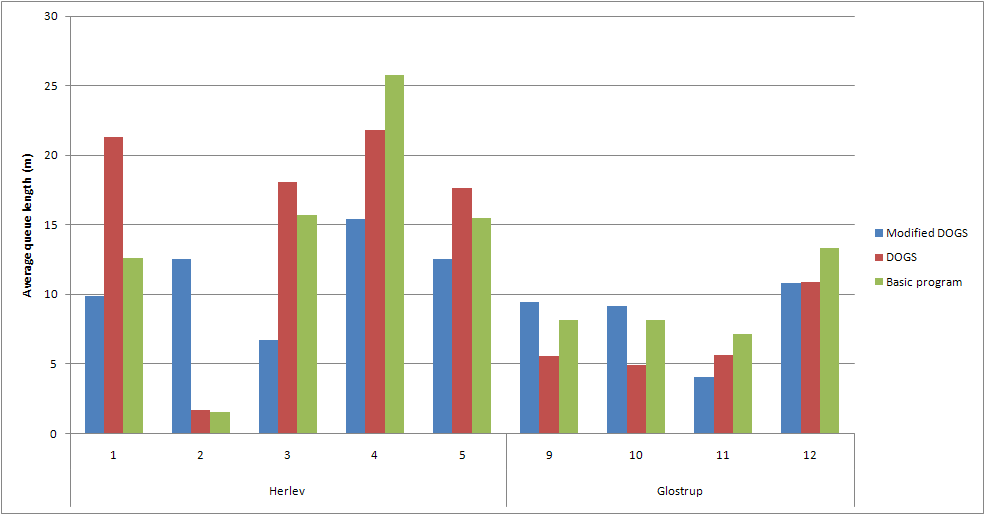
\includegraphics[scale=0.30]{aveq_intersection_arterial.png} 
\end{center}
\caption{Average queue lengths per intersection for arterial traffic}
\label{fig:aveq_int_art}
\end{figure}

\begin{figure}[ht]
\begin{center}
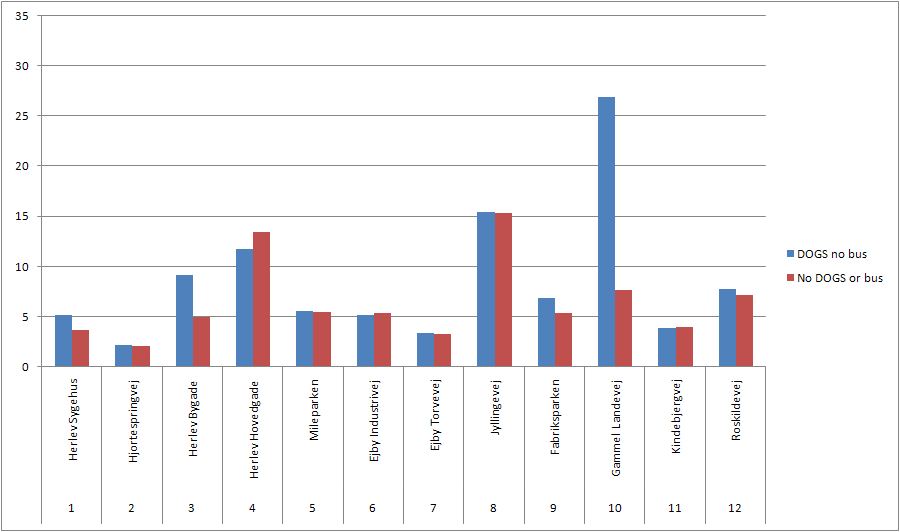
\includegraphics[scale=0.30]{aveq_intersection_total.png} 
\end{center}
\caption{Average queue lengths per intersection for all traffic types}
\label{fig:aveq_int_tot}
\end{figure}

Since intersections 6 to 9 are not controlled by DOGS the performance is almost identical wether DOGS is enabled or not. 

Figure \ref{fig:aveq_int_art} shows the performance queues forming along the arterial. We see that in the Herlev area only arterial traffic at Mileparken gains a slight advantage (~5\%). On the other hand the Herlev Sygehus and Herlev Bygade intersections actually perform more than twice as bad as it did without DOGS. Herlev Hovedgade experience about 5\% longer average queues and Hjortespringvej seems unaffected.

DOGS performs better in all Glostrup intersections yielding from 10\% at Fabriksparken to almost 50\% reduced queue length at Gammel Landevej.

Looking at the performance for crossing traffic, the promised "sacrifices" are clearly visible. In Herlev there are slight increases of average queue length for intersections Herlev Sygehus, Hjortespringvej and Mileparken. Herlev Bygade suffer ~30\% longer queues under DOGS control. Crossing traffic at Herlev Hovedgade, however, actually benefit from DOGS. This can be explained by the fact that the extra cycle time is distributed 4:1 between the main and side directions. Herlev Hovedgade has much crossing traffic and this extra green time will make a difference.

In Glostrup we see moderately decreased performance for Fabriksparken, Kindebjergvej and Roskildevej. Gammel Landevej, however, suffer more than 300\% longer queues on average.

[TODO: HH og GL Landevej vis / henvis til forholdet mellem korridor og non-korridor trafik]

\subsection*{Bus Priority}
In Vissim delays is the difference from the ideal travel time ie. no other vehicles (free flow speeds), no intersections to the actual travel time. 
By this definition the delays experienced at an intersection are correlated with the queue lengths. Unlike queue lengths, Vissim allows us to see delays per vehicle type. This is used to filter out performance for buses.

\begin{figure}[ht]
\begin{center}
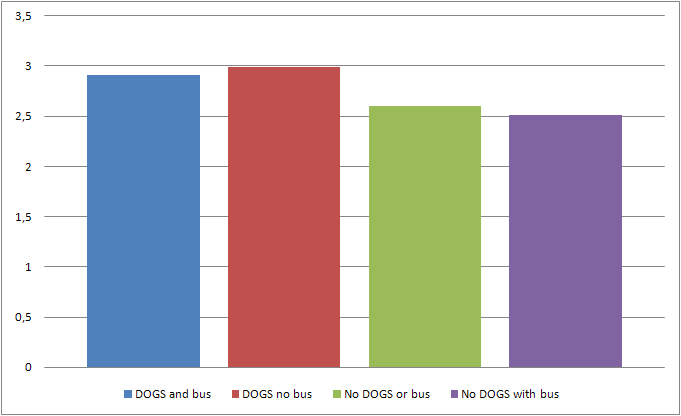
\includegraphics[scale=0.40]{delay_bus.PNG} 
\end{center}
\caption{Total delay for buses in each test case}
\label{fig:bus_delay}
\end{figure}

In Figure \ref{fig:bus_delay} we see how DOGS and bus priority affects bus delays. The worst set of conditions for buses are DOGS enabled and no bus priority while the best occurs without DOGS but with bus priority. 

In both cases, when DOGS is enabled, buses experience more delay than when DOGS is disabled. This could be explained by the increased green time for minor road stages when DOGS increase the cycle time and that buses, when met by a red light, must wait longer than  under a short cycle time.

It is clear that the bus priority logic makes a difference of a few percent reduction in bus delay even though the logic could be more aggressive by detecting waiting buses shortening the non-bus stages so that the stage, which will serve the bus, can start earlier.

\begin{figure}[ht]
\begin{center}
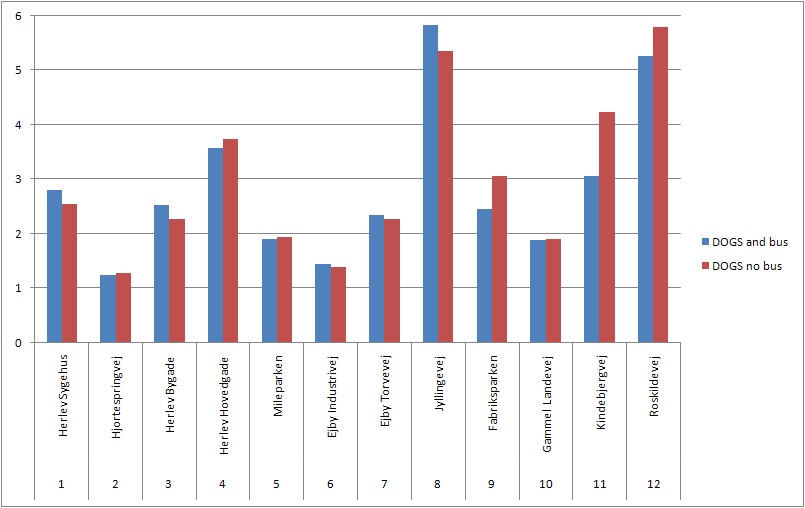
\includegraphics[scale=0.35]{delay_bus_intersection_dogs.PNG} 
\end{center}
\caption{Bus delay per intersection with DOGS}
\label{fig:bus_delay_int_dogs}
\end{figure}

\begin{figure}[ht]
\begin{center}
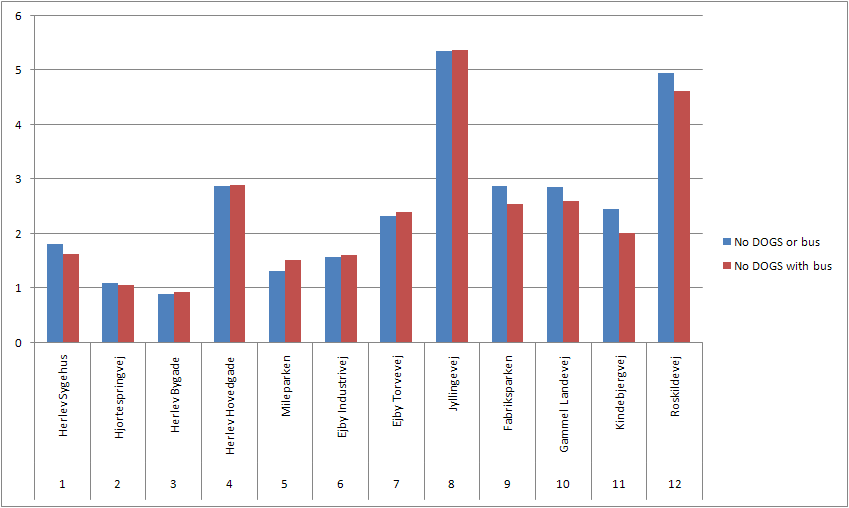
\includegraphics[scale=0.35]{delay_bus_intersection_nodogs.PNG} 
\end{center}
\caption{Bus delay per intersection without DOGS}
\label{fig:bus_delay_int_nodogs}
\end{figure}

In Figures \ref{fig:bus_delay_int_dogs} and \ref{fig:bus_delay_int_nodogs} we see how the bus delay is split over the intersections. In the case with no DOGS the three intersections with bus priority logic perform consistenly better when bus priority is enabled. This is not the case when DOGS is enabled, now only Fabriksparken and Kindebjergvej reduce delays for buses whereas bus delay at Gammel Landevej is indifferent to bus priority. This observation corresponds to what was seen for the average queue lengths for Gammel Landevej in Figure \ref{fig:aveq_int_cross}.

\subsection*{Why DOGS fail in its current incarnation}
These analyses leave an impression of DOGS as a system which work as intended, at best and is detrimental to both arterial and crossing traffic.

We can explain the reason about the observed effects on crossing traffic by the argument of unevenly distributed extra-green time. The case of arterial traffic requires more study, however.

In the DRD report \ref{dogs} Steen Lauritzen makes a note of the uncontrolled behaviour of offsets when DOGS change level (section 5.8). in Figures (\ref{fig:coord_p1_herlev_c80}, \ref{fig:coord_p1_herlev_c100}) we see road time diagrams for the morning program as DOGS increase the common cycle time from 80s to 100s in a time horizon of 300s. 
In the diagram green vertical bands indicate green time for the arterial direction. A platoon of vehicles propagates from the green bands to the next intersection and a red band is drawn when the platoon is met by a red light.

\begin{figure}[ht]

    \begin{minipage}[b]{0.5\linewidth}
    
\begin{center}
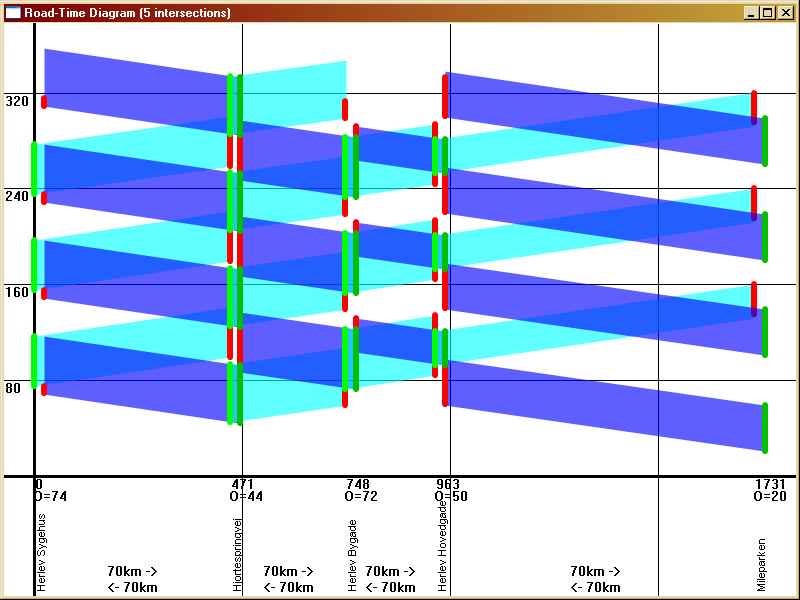
\includegraphics[scale=0.22]{coord_p1_herlev_c80.PNG} 
\end{center}
\caption{Coordination in Herlev without DOGS}
\label{fig:coord_p1_herlev_c80}

    \end{minipage}
    \hspace{0.5cm}
    \begin{minipage}[b]{0.5\linewidth}

\begin{center}
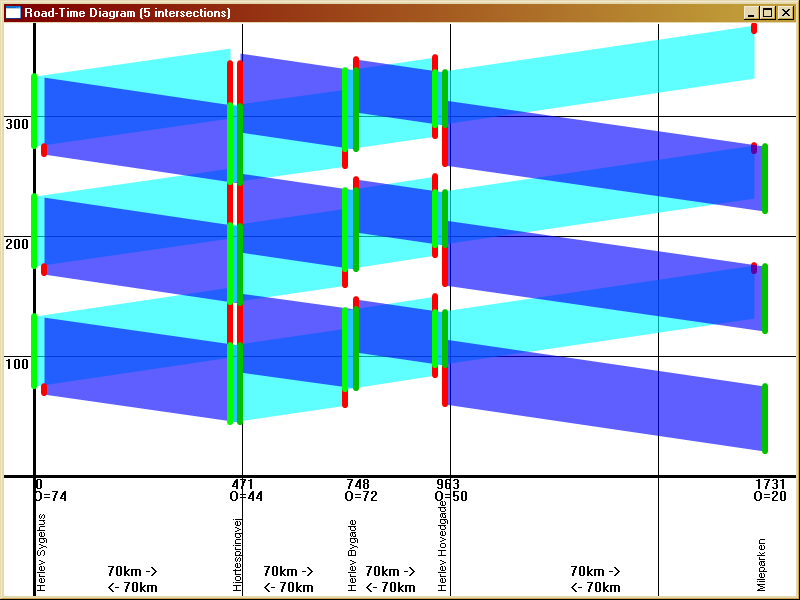
\includegraphics[scale=0.22]{coord_p1_herlev_c100.PNG} 
\end{center}
\caption{Coordination in Herlev at DOGS level 2}
\label{fig:coord_p1_herlev_c100}

    \end{minipage}
    
\end{figure}

We can see how simultaneously extending the green time for the arterial stages will cause the probability for the platoon head of hitting a red light to remain unchanged. This is true because the cycle time is changed at the same time in all intersections (common cycle) and DOGS does not change the red-end times of the arterial stages.
This is also true for the platoon tails, as long as the downstream arterial stage receives the same green time extension as the stage from which the platoon departed.

In the coordination between Herlev Hovedgade and Mileparken we see that DOGS actually \textit{improves} upon the green wave by reducing the probability of meeting a red light going from Herlev Hovedgade to Mileparken at 70km/h.

In Figures (\ref{fig:coord_p1_glostrup_c80} and \ref{fig:coord_p1_glostrup_c100}) we see the same comparison only for the DOGS controller intersections in Glostrup.

\begin{figure}[ht]

    \begin{minipage}[b]{0.5\linewidth}
    
\begin{center}
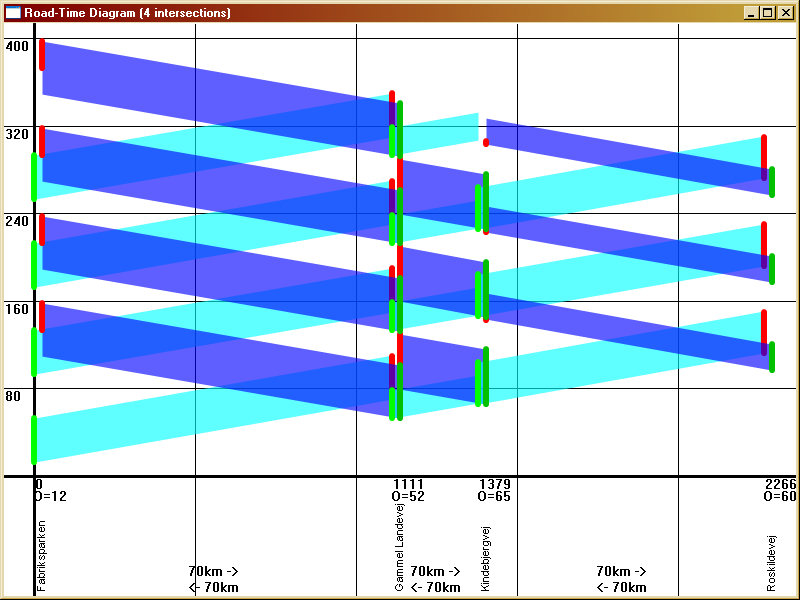
\includegraphics[scale=0.22]{coord_p1_glostrup_c80.PNG} 
\end{center}
\caption{Coordination in Glostrup without DOGS}
\label{fig:coord_p1_glostrup_c80}

    \end{minipage}
    \hspace{0.5cm}
    \begin{minipage}[b]{0.5\linewidth}

\begin{center}
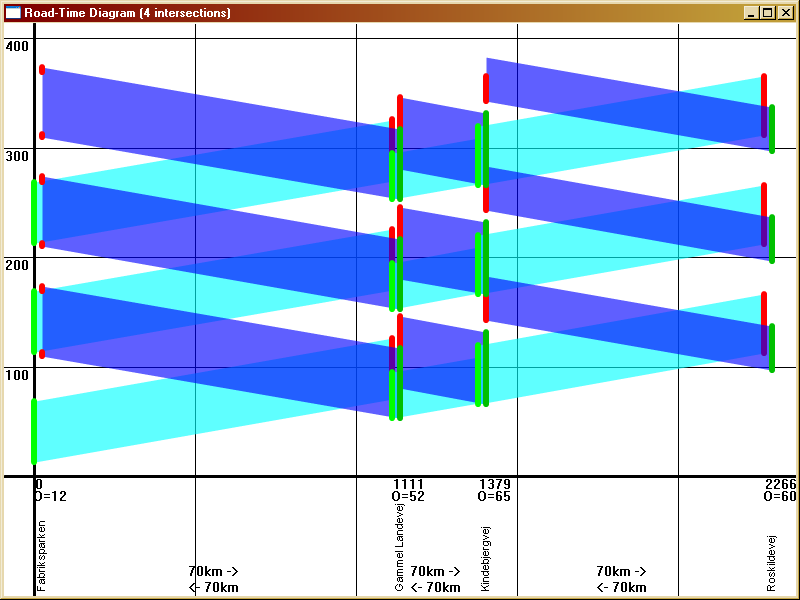
\includegraphics[scale=0.22]{coord_p1_glostrup_c100.PNG} 
\end{center}
\caption{Coordination in Glostrup at DOGS level 2}
\label{fig:coord_p1_glostrup_c100}

    \end{minipage}
    
\end{figure}

[FIX THESE FIGURES - THERE ARE RED BANDS EVEN IN GREEN STARTS!]

We see that with default offsets and cycle time - as well as under DOGS level 2 with cycle time 100s - Gammel Landevej is poorly coordinated with its neighbours, Fabriksparken and Hjortespringvej. Platooons arriving from each of these intersections risk being cut in half at Gammel Landevej. This observation can explain some of poor performance we saw in Figure \ref{fig:aveq_tot} for Gammel Landevej in particular.

During simulation it has been observed how such imperfect coordinations are affected by DOGS; more vehicles are stopped at the red light due to the increased capacity and queues become longer.

\subsection{DOGS with level-specific offsets}
In the previous section we saw that the performance of DOGS is unreliable when adjusting the cycle time with adjust the coordination by changing the offsets.

To show that incorrect offsets are indeed the problem with the original DOGS I use the optimization routine described in section \ref{optimization} to precalculate cycle-time specific offsets for each DOGS-controller signal controller. While original DOGS allows level changes after one cycle has passed, DOGS with cycle-time specific offsets was reprogrammed to wait at least 3 cycles before changing levels to allow the new offsets to come into effect.

\subsection{Coordination with Direction Priority Offsets}
In this test the system for coordination of section \ref{coordination} is compared with DOGS without bus priority. DRD requested this test to discover whether DOGS (dynamic capacity) can outperform a proper coordination. DOGS has support for dynamically adjusting the coordination - including prioritizing directions - though it is not enabled in either the Glostrup or Herlev sites at the moment.

